% Architecture figure. Compile separately: pdflatex architecture.tex
% Layout is on an explicit coordinate grid (cm). Four bands, all reading left to right:
%   y =  0.0   perception : input views -> frozen encoder -> camera-aware tokens -> decoder
%   y = -2.9   heads      : direct head | object control-point head | joint head
%   y = -5.6   geometry   : canonical mesh -> Procrustes -> soft nearest vertex
%   y = -8.15  output     : precision-weighted fusion -> predicted field on the reference view
% Columns are aligned across bands (x = 2.8 / 10.8 / 17.5) so no wire crosses a box.
% Every box carries a 5.4 mm pictogram of what it computes, drawn in the box's own accent colour.
\documentclass[tikz,border=2pt]{standalone}
\usepackage{amsmath,amssymb,xcolor,graphicx,helvet}
\renewcommand{\familydefault}{\sfdefault}
% Notation (docs/07): keep consistent across text, figures and tables.
\newcommand{\PaperTitle}{Factored Interaction Fields: Learning Joint-Anchored Hand-Object Proximity Through Its Geometric Arguments}
\newcommand{\method}{FIF}
\newcommand{\field}{\mathbf{v}}
\newcommand{\joint}{\mathbf{p}}
\newcommand{\vtx}{\mathbf{q}}
\newcommand{\objpose}{\theta_o}
\newcommand{\Rot}{\mathbf{R}}
\newcommand{\trans}{\mathbf{t}}
\newcommand{\mesh}{\mathcal{Q}}
\newcommand{\ade}{\mathrm{ADE}}
\newcommand{\mm}{\,\mathrm{mm}}
\newcommand{\ie}{i.e.}
\newcommand{\eg}{e.g.}

\usetikzlibrary{arrows.meta,fit,backgrounds,calc}

\definecolor{cfroz}{HTML}{6E6E6E}\definecolor{cfrozf}{HTML}{EFEFEF}
\definecolor{ctrain}{HTML}{3C6E9F}\definecolor{ctrainf}{HTML}{E5EDF6}
\definecolor{cgeo}{HTML}{2E7D4F}\definecolor{cgeof}{HTML}{E5F1E9}
\definecolor{cfuse}{HTML}{C1692C}\definecolor{cfusef}{HTML}{FBEDE1}
\definecolor{closs}{HTML}{BF3B2B}\definecolor{cwire}{HTML}{4D4D4D}
\newcommand{\m}[1]{\mbox{$#1$}}
\newcommand{\s}[1]{{\scriptsize #1}}

% ---------------------------------------------------------------- pictograms (5.4 x 5.4 mm each)
\newcommand{\ICO}[1]{\begin{tikzpicture}[baseline=(current bounding box.center),x=0.9mm,y=0.9mm,
  line width=0.4pt,line cap=round,line join=round,sharp corners]\useasboundingbox (-0.15,-0.15) rectangle (6.15,6.15);#1\end{tikzpicture}}
\newcommand{\tip}{-{Latex[length=1.2mm,width=1.0mm]}}

% frozen encoder: a grid of image patches, marked frozen by a snowflake
\newcommand{\iconFrozen}{\ICO{%
  \foreach \i in {0,1,2}{\foreach \j in {0,1,2}{%
    \draw[cfroz!70,fill=cfroz!22] (0.15+\i*1.6,0.15+\j*1.6) rectangle ++(1.45,1.45);}}%
  \fill[white] (4.6,4.6) circle (1.75);
  \foreach \a in {0,60,120}{\draw[cfroz,line width=0.5pt] (4.6,4.6) +(\a:1.5) -- +({\a+180}:1.5);}%
  \fill[cfroz] (4.6,4.6) circle (0.32);
}}

% camera-aware tokens: viewing rays from the camera centre tagging patch tokens
\newcommand{\iconTokens}{\ICO{%
  \foreach \y in {0.85,3.0,5.15}{%
    \draw[ctrain!85] (0.55,3) -- (4.7,\y);
    \draw[ctrain,fill=ctrain!45,line width=0.35pt] (4.7,{\y-0.6}) rectangle ++(1.2,1.2);}%
  \fill[ctrain] (0.55,3) circle (0.5);
}}

% transformer decoder: queries attending to memory tokens
\newcommand{\iconDecoder}{\ICO{%
  \foreach \a/\b in {0.9/0.7,0.9/2.5,3.0/2.5,3.0/4.3,5.1/4.3,5.1/5.7,3.0/0.7}{%
    \draw[ctrain!50,line width=0.3pt] (\a,4.85) -- (\b,1.15);}%
  \foreach \x in {0.9,3.0,5.1}{\fill[ctrain] (\x,5.3) circle (0.5);}%
  \foreach \x in {0.7,2.5,4.3,5.7}{\draw[ctrain,fill=white,line width=0.35pt] (\x,0.7) circle (0.42);}%
}}

% direct head: one vector regressed straight out, with its predicted uncertainty
\newcommand{\iconDirect}{\ICO{%
  \draw[ctrain!55,dash pattern=on 0.45mm off 0.32mm,line width=0.35pt] (4.4,4.4) circle (1.35);
  \draw[ctrain,\tip,line width=0.55pt] (1.15,1.25) -- (4.4,4.4);
  \fill[ctrain] (1.15,1.25) circle (0.5);
}}

% object control-point head: control points sampled on the object
\newcommand{\iconCtrl}{\ICO{%
  \begin{scope}[shift={(3,3)}]
    \draw[ctrain,fill=ctrain!14] (90:2.35) -- (162:2.35) -- (234:2.35) -- (306:2.35) -- (18:2.35) -- cycle;
    \foreach \a in {90,162,234,306,18}{\draw[ctrain] (0,0) -- (\a:2.35);}
    \foreach \a in {90,162,234,306,18}{\fill[ctrain] (\a:2.35) circle (0.55);}
    \fill[ctrain!60] (0,0) circle (0.45);
  \end{scope}}}

% joint head: the hand skeleton
\newcommand{\iconJoint}{\ICO{%
  \draw[ctrain,line width=0.45pt] (3,0.7) -- (1.25,2.35) -- (0.8,3.9) -- (0.7,5.3);
  \draw[ctrain,line width=0.45pt] (3,0.7) -- (3,2.5) -- (3,4.0) -- (3,5.45);
  \draw[ctrain,line width=0.45pt] (3,0.7) -- (4.75,2.35) -- (5.2,3.9) -- (5.3,5.3);
  \foreach \p in {(3,0.7),(1.25,2.35),(0.8,3.9),(0.7,5.3),(3,2.5),(3,4.0),(3,5.45),(4.75,2.35),(5.2,3.9),(5.3,5.3)}{%
    \fill[ctrain] \p circle (0.38);}%
}}

% weighted Procrustes: a canonical point set rotated onto the predicted one
\newcommand{\iconProc}{\ICO{%
  \draw[cgeo!55,densely dashed,line width=0.35pt] (0.7,0.9) -- (2.7,0.6) -- (1.7,2.7) -- cycle;
  \foreach \p in {(0.7,0.9),(2.7,0.6),(1.7,2.7)}{\draw[cgeo!70,fill=white,line width=0.35pt] \p circle (0.42);}%
  \draw[cgeo] (3.4,3.2) -- (5.5,3.6) -- (4.4,5.5) -- cycle;
  \foreach \p in {(3.4,3.2),(5.5,3.6),(4.4,5.5)}{\fill[cgeo] \p circle (0.45);}%
  \draw[cgeo,\tip,line width=0.45pt] (1.85,3.5) to[bend left=32] (3.2,4.75);
}}

% soft nearest vertex: a joint, the object surface, and the soft neighbourhood of the nearest vertex
\newcommand{\iconSoftNN}{\ICO{%
  \draw[cgeo,line width=0.5pt] (0.3,4.3) -- (1.7,5.3) -- (3.2,4.2) -- (4.6,5.2) -- (5.8,4.2);
  \draw[cgeo!45,densely dashed,line width=0.35pt] (3.2,4.2) circle (1.2);
  \foreach \p in {(0.3,4.3),(1.7,5.3),(3.2,4.2),(4.6,5.2),(5.8,4.2)}{\fill[cgeo] \p circle (0.4);}%
  \draw[cgeo,\tip,line width=0.55pt] (2.45,0.85) -- (3.13,3.55);
  \fill[ctrain] (2.45,0.85) circle (0.5);
}}

% precision-weighted fusion: a sharp and a broad estimate combined, the mean pulled to the sharp one
\newcommand{\iconFusion}{\ICO{%
  \draw[black!25,line width=0.3pt] (0.2,0.55) -- (5.8,0.55);
  \draw[cgeo,line width=0.5pt] plot[domain=0.2:5.8,samples=34,smooth] (\x,{0.55+1.65*exp(-pow(\x-3.8,2)/3.4)});
  \draw[ctrain,line width=0.5pt] plot[domain=0.2:5.8,samples=34,smooth] (\x,{0.55+4.1*exp(-pow(\x-2.35,2)/0.55)});
  \draw[cfuse,line width=0.6pt] (2.75,0.3) -- (2.75,5.3);
  \fill[cfuse] (2.75,5.3) circle (0.4);
}}

% box content: pictogram on the left, centred text block on the right
\newcommand{\bx}[2]{#1\hspace{1.3mm}\begin{tabular}{@{}c@{}}#2\end{tabular}}

\begin{document}
\renewcommand{\arraystretch}{1.12}
\begin{tikzpicture}[x=1cm,y=1cm,
  box/.style={draw, rounded corners=2pt, line width=0.55pt, inner xsep=4pt, inner ysep=4pt, font=\footnotesize},
  frozen/.style={box, fill=cfrozf, draw=cfroz},
  train/.style={box, fill=ctrainf, draw=ctrain},
  geo/.style={box, fill=cgeof, draw=cgeo},
  fuse/.style={box, fill=cfusef, draw=cfuse},
  asset/.style={inner sep=0, draw=black!35, line width=0.4pt},
  arr/.style={-{Latex[length=1.9mm,width=1.5mm]}, line width=0.6pt, draw=cwire},
  wire/.style={line width=0.6pt, draw=cwire},
  lbl/.style={font=\scriptsize, text=black!60, inner sep=1.5pt, align=center},
  loss/.style={font=\scriptsize, text=closs, align=left, inner sep=1pt},
]

% ================================================== band 1: perception (y = 0)
\node[asset] (img0) at (0.78,0) {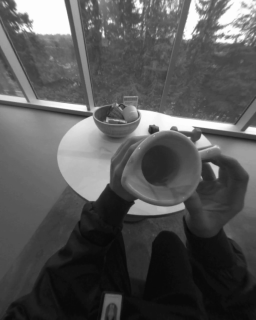
\includegraphics[width=11mm]{thumb_in0.png}};
\node[asset] (img1) at (2.12,0) {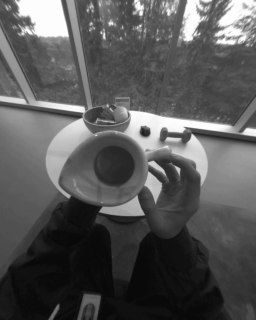
\includegraphics[width=11mm]{thumb_in1.png}};
\node[lbl, anchor=north] at (1.45,-0.80) {two synchronised headset views\\$1024{\times}1280$, known calibration};
\node[frozen, minimum width=33mm, minimum height=15mm] (enc) at (5.50,0)
  {\bx{\iconFrozen}{frozen encoder\\\s{DINOv3 ViT-B/16}\\\s{$2{\times}720$ patch tokens}}};
\node[train, minimum width=56mm, minimum height=15mm] (tok) at (10.80,0)
  {\bx{\iconTokens}{camera-aware tokens\\\s{\m{\mathbf{X}'_v=\mathbf{P}\mathbf{X}_v+\mathrm{MLP}(\boldsymbol{\pi})+\mathbf{e}_{\rm view}+\mathbf{e}_{\rm pos}}}\\\s{$\boldsymbol{\pi}$: Pl\"ucker ray of the token}}};
\node[train, minimum width=54mm, minimum height=15mm] (dec) at (17.50,0)
  {\bx{\iconDecoder}{transformer decoder\\\s{$L{=}6$ layers, self- and cross-attention}\\\s{42 joint $+$ 16 object queries}}};
\draw[arr] (img1.east) -- (enc.west);
\draw[arr] (enc.east) -- node[lbl, above=0.2mm] {cached} (tok.west);
\draw[arr] (tok.east) -- node[lbl, above=0.2mm] {memory} (dec.west);

% ================================================== band 2: heads (y = -2.9)
\node[train, minimum width=50mm, minimum height=10mm] (hdir) at (2.80,-2.90)
  {\bx{\iconDirect}{direct head\\\s{field \m{\field^{\rm dir}_{h,j}}, log-scale \m{s^{\rm dir}_{h,j}}}}};
\node[train, minimum width=54mm, minimum height=10mm] (hobj) at (10.80,-2.90)
  {\bx{\iconCtrl}{object control-point head\\\s{points \m{\hat{\mathbf{c}}_n}, confidences \m{w_n}}}};
\node[train, minimum width=54mm, minimum height=10mm] (hjnt) at (17.50,-2.90)
  {\bx{\iconJoint}{joint head\\\s{camera-frame joints \m{\hat{\joint}_{h,j}} (mm)}}};
% query bus: one drop from the decoder, one horizontal channel, three taps
\draw[wire] (dec.south) -- (17.50,-1.95);
\draw[wire] (2.80,-1.95) -- (17.50,-1.95);
\draw[arr] (2.80,-1.95) -- (hdir.north);
\draw[arr] (10.80,-1.95) -- (hobj.north);
\draw[arr] (17.50,-1.95) -- (hjnt.north);
\node[lbl, anchor=south] at (14.35,-1.90) {refined queries};

% ================================================== band 3: geometry (y = -5.6)
\node[inner sep=0] (mesh) at (2.60,-5.55) {\includegraphics[width=13mm]{thumb_mesh.png}};
\node[lbl, anchor=west, align=left] (meshl) at (3.45,-5.55)
  {canonical mesh $\mesh_a$\\(object alias given)\\16 control points $\mathbf{c}_n$\\1{,}024 vertices $\vtx_m$};
\node[geo, minimum width=54mm, minimum height=13mm] (proc) at (10.80,-5.60)
  {\bx{\iconProc}{weighted Procrustes alignment\\\s{\m{\arg\min\nolimits_{\Rot,\trans}\sum_n w_n\lVert\Rot\mathbf{c}_n+\trans-\hat{\mathbf{c}}_n\rVert^2}}\\\s{closed form, differentiable through the SVD}}};
\node[geo, minimum width=54mm, minimum height=13mm] (snn) at (17.50,-5.60)
  {\bx{\iconSoftNN}{soft nearest vertex on the posed mesh\\\s{\m{\hat{\vtx}_m=\hat{\Rot}_o\vtx_m+\hat{\trans}_o},\ \ \m{w_{jm}\propto e^{-\lVert\hat{\vtx}_m-\hat{\joint}_j\rVert^2/\tau}}}\\\s{\m{\field^{\rm geo}_j=\sum_m w_{jm}\hat{\vtx}_m-\hat{\joint}_j},\ \ \m{\tau:400\to25\,\mathrm{mm}^2}}}};
\draw[arr] (hobj.south) -- (proc.north);
\draw[arr] (meshl.east) -- (proc.west);
\draw[arr] (proc.east) -- (snn.west);
\draw[arr] (hjnt.south) -- node[lbl, right=0.4mm] {\m{\hat{\joint}_{h,j}}} (snn.north);

% ================================================== band 4: fusion and output (y = -8.15)
\node[fuse, minimum width=88mm, minimum height=12mm] (fus) at (7.20,-8.15)
  {\bx{\iconFusion}{precision-weighted fusion\\\s{\m{\hat{\field}_{h,j}=\dfrac{\lambda^{\rm dir}\field^{\rm dir}_{h,j}+\lambda^{\rm geo}\field^{\rm geo}_{h,j}}{\lambda^{\rm dir}+\lambda^{\rm geo}}},\qquad \m{\lambda^{k}_{h,j}=e^{-2s^{k}_{h,j}}}}}};
\node[asset] (out) at (16.00,-8.15) {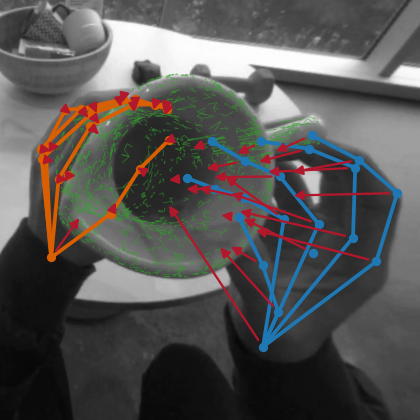
\includegraphics[width=25mm]{thumb_out.png}};
\node[lbl, anchor=north, align=center] at (16.00,-9.50) {predicted field (red) on the reference\\view; $2{\times}21{\times}3$ (mm), world frame};
% direct head down the left rail into the fusion
\draw[wire] (1.40,-3.40) -- (1.40,-8.15);
\draw[arr] (1.40,-8.15) -- (fus.west);
\node[lbl, anchor=west] at (1.52,-6.95) {\m{\field^{\rm dir}, s^{\rm dir}}};
% geometric estimate into the fusion
\draw[wire] (16.00,-6.25) -- (16.00,-7.05) -- (10.80,-7.05);
\draw[arr] (10.80,-7.05) -- (10.80,-7.55);
\node[lbl, anchor=south] at (13.40,-7.03) {\m{\field^{\rm geo}, s^{\rm geo}}};
\draw[arr] (fus.east) -- node[lbl, above=0.2mm] {\m{\Rot_{w\leftarrow c}}} (out.west);

% ================================================== losses
\node[loss, anchor=north west] at (1.65,-3.85)
  {auxiliary losses on the heads:\\$\mathcal{L}_{\rm joint}$ (\mbox{$\ell_1$}), $\mathcal{L}_{\rm obj}$ (\mbox{ADD-S}), $\mathcal{L}_{\rm vis}$, $\mathcal{L}_{\rm pres}$ (BCE);\\also on frames with only a hand or only an object};
\node[loss, anchor=south west] at (2.90,-7.48)
  {$\mathcal{L}_{\rm field}$ (ADE of $\hat{\field}$) $+\ \lambda_{\rm dir}\mathcal{L}^{\rm NLL}_{\rm dir}+\lambda_{\rm geo}\mathcal{L}^{\rm NLL}_{\rm geo}$};

% ================================================== legend
\begin{scope}[shift={(18.05,-7.45)}]
  \node[frozen, minimum width=5mm, minimum height=2.4mm, inner sep=0] (k1) at (0,0) {};
  \node[lbl, anchor=west, text=black!70] at (0.34,0) {frozen};
  \node[train, minimum width=5mm, minimum height=2.4mm, inner sep=0] (k2) at (0,-0.40) {};
  \node[lbl, anchor=west, text=black!70] at (0.34,-0.40) {trained};
  \node[geo, minimum width=5mm, minimum height=2.4mm, inner sep=0] (k3) at (0,-0.80) {};
  \node[lbl, anchor=west, text=black!70] at (0.34,-0.80) {geometry};
  \node[fuse, minimum width=5mm, minimum height=2.4mm, inner sep=0] (k4) at (0,-1.20) {};
  \node[lbl, anchor=west, text=black!70] at (0.34,-1.20) {fusion};
  \node[lbl, anchor=west, text=closs] at (0,-1.60) {red: losses};
\end{scope}
\end{tikzpicture}
\end{document}
